\documentclass[12pt,a4paper,margin=1in]{book}
\usepackage[utf8]{inputenc}
\usepackage{amsmath}
\usepackage{amsfonts}
\usepackage{amssymb}
\usepackage{graphicx}
\usepackage{braket}
\usepackage{bm}
\begin{document}

\chapter{Theory of Laser Spectroscopy}
Note: Throughout this section, a variable written in a bold typeface is vector valued, while its non-bold counterpart is its magnitude. 
\section{Anatomy of A Hyperfine Spectrum}
\begin{figure}[h]
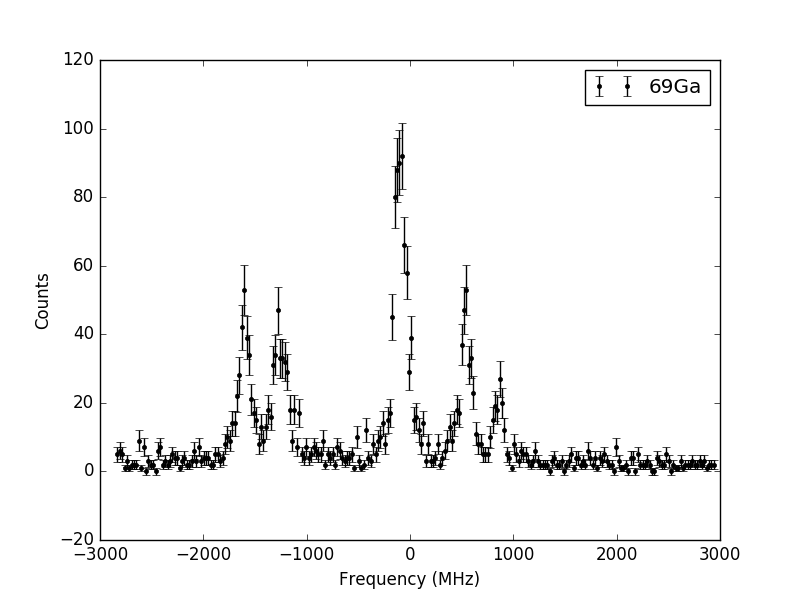
\includegraphics[width=\textwidth]{Graphics/ga69.png}
\label{ga69}
\end{figure}
How can the properties of a hyperfine spectrum, such as that of $^{69}\mathrm{Ga}$ shown in Fig. \ref{ga69}, be translated into measurements of the physical properties of the nucleus? The hyperfine spectrum is, after all, the result of probing the electronic structure of the atom. The answer, of course, is that the electrons interact with the nucleus through several mechanisms, each of which will be described in this section. To begin, however, consider the following system: An electron transitions from a ground state $\ket{g}$ to an excited state $\ket{e}$. More precisely $\ket{g}$ and $\ket{e}$ are defined as 
\begin{align}
\ket{g} =& \ket{n_g,J_g,J_g^z}\\
\ket{e} =& \ket{n_e,J_e,J_e^z}
\end{align}
where $n_{g,e}$ are principal quantum numbers, $\bf{J_{g,e}}$ the orbital angular momenta, and $J_{g,e}^z$ the projections of the orbital angular momentum on an axis of quantization $z$. Next, if nucleus of the atom in which this transition is occurring has angular momentum $\bf{I}$, then a quantity, $\bf{F}$, can be defined as 

\begin{equation}
\bf{F_{g,e}} = \bf{I} + \bf{J_{g,e}}
\end{equation}

$\bf{F}$ describes the total angular momentum state of the atom, so $\ket{g}$ and $\ket{e}$ can be rewritten as

\begin{align}
\ket{g} =& \ket{n_g,\mathrm{F_g}}\\
\ket{e} =& \ket{n_e,\mathrm{F_e}}
\end{align}

For a fixed $\bf{I}$, $\bf{F}$ can range from $(-\mathrm{J}+I)$ to $(\mathrm{J}+I)$.
\subsection{Peak Energies}
The energy of the electrons depends on the various electron-nucleus interactions present in the atom. If for the purposes of this work, only three interactions produce measurable changes in the energies of the electron levels. These are the isotope, magnetic dipole and electric quadrupole shifts. There are higher order interactions (magnetic octopole, electric sixteen-o-pole), however their effects are far below the resolution of the experimental set-up employed at TRIUMF. For example, the three interactions listed above lead to energy shifts on the order of an eV. Higher order interactions are (CITATION AND ANSWER NEEDED) 

\subsubsection*{Isotope Shift}
The isotope shift is measured with respect to a reference isotope. As neutrons are added or removed from a nucleus, the charge distribution, as well as the mass, of the nucleus changes. This leads to three different effects on the energies of the electrons. 

The change in the mass of the nucleus leads to what is known as the Mass shift, $\Delta E_M$. The mass shift between two isotopes with mass numbers A and A' is given by
\begin{equation}
\Delta E_M = \frac{m_{\mathrm{A}}-m_{\mathrm{A'}}}{2 m_{\mathrm{A}} m_{\mathrm{A'}}} \left(\sum_i\mathrm{\textbf{p}}_i +2 \sum_{i>j}\mathrm{\textbf{p}}_i \cdot \mathrm{\textbf{p}}_j \right)
\end{equation}
where $m_{\mathrm{A}}$ and $m_{\mathrm{A'}}$ are the isotope masses, and the $\textbf{p}_i$ are the electron momenta. The first term is due to the nucleus recoiling with the electrons when a photon is absorbed, while the second term deals with the electron-electron interactions.  

The change in the charge distribution of the nucleus produces the Field shift. While the typical nucleus is far smaller the wavefunction of a typical orbital electron, the effect is still important. The energy of a nucleus in the charge density produced by the electrons at the origin, $E_F$, is given by

\begin{equation}
E_F = \frac{Ze^2}{6 \epsilon_0}|\psi(0)|^2 \left\langle r_{ch}^2\right\rangle
\end{equation}
where $\epsilon_0$ is the permitivity of free space, $Z$ is the proton number and $ \left\langle r_{ch}^2\right\rangle$ is the mean-square charge radius of the nucleus, defined as
\begin{equation}
 \left\langle r_{ch}^2\right\rangle = \frac{\int_0^{\infty}\rho(\mathbf{r})r^2dV}{\int_0^{\infty}\rho(\mathbf{r})dV}
\end{equation}
The field shift between two isotopes is then given by
\begin{equation}
\Delta E_F =  \frac{Ze^2}{6 \epsilon_0}\Delta|\psi(0)|^2 \Delta\left\langle r_{ch}^2\right\rangle
\end{equation}

In total, then, the isotope shift $\Delta E_{\mathrm{A,A}'}$ is given by
\begin{equation}
 \Delta E_{\mathrm{A,A'}} = \Delta E_M + \Delta E_F
\end{equation}
\subsubsection*{Magnetic Dipole Shift}
A nucleus with a non-zero nuclear spin $\bf{I}$  will have a magnetic dipole moment, given by

\begin{equation}
\boldsymbol{\mu}_{\mathrm{\bf{I}}} = g_{\mathrm{I}}\mu_{\mathrm{N}}\mathrm{\bf{I}}
\end{equation}

where $g_{\mathrm{I}}$ is the g-factor and $\mu_{\mathrm{N}}$ is the nuclear magneton. (REFERENCE NEEDED) The interaction of $\mu_{\mathrm{I}}$ with the magnetic field produced by the electrons, $\mathrm{\bf{B_e}}$, creates a shift in the energy of the orbiting electrons. Provided the electrons occupy an angular momentum state $\mathrm{\bf{J}} \neq 0$, the hamiltonian for this interaction is given by

\begin{equation}
\mathcal{H} = -\boldsymbol{\mu}_{\mathrm{\bf{I}}} \cdot \mathrm{\bf{B_e}}
\end{equation}

This interaction leads to a shift, $\Delta E_{\mu_I}$, in the energy of the atomic states by

\begin{equation}
\Delta E_{\mu_I} = \frac{AK}{2}
\end{equation}

where $K = \mathrm{F(F+1) - I(I+1) - J(J+1)}$ and 

\begin{equation}
A = \frac{\mu_{\mathrm{I}}\mathrm{B_e}}{\mathrm{IJ}}
\end{equation}

\subsubsection*{Electric Quadrupole Shift}
The electric quadrupole moment is used to describe the distribution of charge in a nucleus. For a nucleus composed of $n$ protons and $\mathbf{I}\geq1$, the electric quadrupole moment, Q, is given by

\begin{equation}
\mathrm{Q} = \sum_i^n (3z_i^2-r_i^2)
\end{equation}
where $r_i^2 = x_i^2+y_i^2+z_i^2$. If Q $ < 0$, then the nucleus is stretched in the $x-y$ plane. If Q $ > 0$, then the nucleus is stretched along the $z-$axis. It is important to note that these deformations a symmetric with respect to an axis of symmetry, the $z-$axis in this case. Q $=0$ indicates that the nucleus is spherical. 

In reality, direct measurement of Q is not feasible, as the nucleus is rotating. Instead, the spectroscopic quadrupole, Q$_s$, is measured. Q$_s$ is defined as the projection of Q onto the axis of quantization of the nucleus, and is given by
\begin{equation}
\mathrm{Q}_s = \frac{\mathrm{I}(2\mathrm{I}-1)}{(\mathrm{I}+1)(2\mathrm{I}+3)}\mathrm{Q}
\end{equation}
The use of $Q_s$ as a measure of $Q$ is valid under the assumption that the nuclear deformation is axially symmetric. Additionally, it is assumed that the axis of symmetry has a well defined direction with respect to \textbf{I}.

The hamiltonian for the interaction between the spectroscopic electric quadrupole moment and the electric field produced by the electrons at the nucleus, $E_N$, is given by

\begin{equation}
\mathcal{H} = - \frac{1}{6}e\mathrm{Q}_s\nabla{E_N}
\end{equation}
where
\begin{equation}
\nabla{E_N} = \frac{\partial^2V}{\partial x_i\partial x_j}, \{x_j,x_k\} \in \{x,y,z\} \otimes \{x,y,z\}
\end{equation}
$e$ is the fundamental charge and $V$ is the electric potential. Recalling that the nuclear deformation is symmetric about the axis of quantization, the shift in energy is then given by

\begin{equation}
\Delta E_{\mathrm{Q_s}} = \frac{B}{4}\left[\frac{\frac{3}{2}K(K+1)-2\mathrm{I}(\mathrm{I}+1)\mathrm{J}(\mathrm{J}+1)}{\mathrm{I}(2\mathrm{I}-1)\mathrm{J}(2\mathrm{J}-1)}\right]
\end{equation}
where $B$ is a hyperfine coefficient and is given by
\begin{equation}
B = e\mathrm{Q_s}\left\langle\frac{\partial^2V}{\partial z^2} \right\rangle
\end{equation}

\subsubsection*{The Hyperfine Equation}
The resonant energy of a transition between $\ket{g}=\ket{n_g,\mathrm{\textbf{F}_g=\textbf{I} + \textbf{J}_g}}$ and $\ket{e}=\ket{n_e,\mathrm{\textbf{F}_e=\textbf{I} + \textbf{J}_e}}$ is then given by
\begin{equation}
E_{hfs} = E_{fs} +  \Delta E_{\mathrm{A,A'}}+\Delta E_{\mu_I}\Bigr|_{\mathrm{F_g},I,J_g}^{\mathrm{F_e},I,J_e}+\Delta E_{\mathrm{Q_s}}\Bigr|_{\mathrm{F_g},I,J_g}^{\mathrm{F_e},I,J_e}
\end{equation}

\begin{equation}
\Delta E_{hfs} = 
\end{equation}
\end{document}